\documentclass[14pt, a4paper]{report}
\usepackage{mathtext}
\usepackage[T2A]{fontenc}
\usepackage[utf8]{inputenc}
\usepackage[russian]{babel}
\usepackage{multirow}
\usepackage{slashbox}
\usepackage{makecell}
\usepackage{graphicx}
\usepackage{physics}
\usepackage{amstext}
\usepackage{caption}
\usepackage{subcaption}

\renewcommand{\thesection}{\arabic{section}.}
\renewcommand{\thesubsection}{\arabic{section}.\arabic{subsection}.}

\title{\textbf{Отчет о выполнении лабораторной работы 3.1.3 "Измерение магнитного поля Земли"}}
\author{Калашников Михаил, Б03-205}
\date{}

\begin{document}
\maketitle

\textbf{Цель работы:}
исследовать свойства постоянных неодимовых магнитов; измерить с их помощью горизонтальную и вертикальную составляющие индукции магнитного поля Земли и магнитное наклонение.
\newline

\textbf{В работе используются:}
\begin{itemize}
\item неодимовые магниты;
\item тонкая нить, закрепленная на штативе;
\item медная проволока;
\item электронные весы ($\sigma_m=0.001\ г$);
\item секундомер ($\sigma_t=0.01\ с$);
\item измеритель магнитной индукции;
\item штангенциркуль ($\sigma_d=0.1\ мм$);
\item микрометр ($\sigma_d=0.01\ мм$);
\item деревянные бруски;
\item набор гирь.
\end{itemize}

\section{Теоретические сведения}

Магнитный диполь может быть образован постоянным магнитом или витком с током. Такой диполь описывается величиной $\overline{P}$ -- магнитным моментом. Он всегда направлен от южного полюса магнита к северному. Если размеры диполя малы по сравнению с расстоянием до него, то такой диполь называют точечным.
Магнитное поле точечного диполя определяется по формуле (в СГС):
\[\overline{B}=\frac{3\left(\overline{P}\cdot\overline{r}\right)\overline{r}}{r^5}-\frac{\overline{P}}{r^3}\]

Если точечный магнитный диполь поместить во внешнее магнитное поле с индукцией $\overline{B}$, то на него будет действовать механический момент сил:
\[\overline{M}=\left[\overline{P}\cross\overline{B}\right]\]

Потенциальная энергия, которой обладает такой диполь будет определяться следующим образом:
\[W=-\left(\overline{P}\cdot\overline{B}\right)\]

Из этого следует, что диполь будет находиться в состоянии устойчивого равновесия тогда и только тогда, когда его магнитный момент будет сонаправлен с индукцией внешнего магнитного поля.

Сила взаимодействия между двумя диполями с моментами $\overline{P_1}$ и $\overline{P_2}$ на расстоянии $r$ друг от друга может быть рассчитана по формуле:
\[\overline{F}=-\frac{6\overline{P_1}\overline{P_2}}{r^4}\] 

\section{Экспериментальная установка}

Установка представляет из себя штатив с закрепленной на нем нитью. К нити можно приклеплять различные конструкции из неодимовых магнитов.

Рассмотрим крутильные колебания "стрелки" из магнитных шариков. Не учитывая силы, возникающие в нити, при отклонение стрелки на угол $\theta$, на маятник начинает действовать возвращающий момент сил:
\[M=-P_nB_{гор}\sin{\theta}\]
При малых углах отклонения, уравнение колебаний имеет вид:
\[I_n\ddot{\theta}+P_nB_{гор}\theta=0\]
Представляя цепочку магнитов тонким однородным стержнем ($I_n=\frac{1}{12}n^3md^2$), выражаем период таких колебаний:
\[T=\pi\sqrt{\frac{md^2}{3PB_{гор}}}\cdot n\]

Теперь рассмотрим ту же "стрелку", но закрепленную на нити в одной точке. В магнитном поле Земли, которое отклонено от горизонтали на угол $\beta$, цепочка тоже отклонится на определенный угол. Уравновесив ее дополнительным грузом $m_{гр}$, можно определить велчиниу вертикальной составляющей магнитного поля.
\[M_n=m_{гр}gr_{гр}=nPB_{верт}\]

\section{Проведение эксперимента и обработка данных}

\begin{enumerate}

\setcounter{enumi}{0}

\item Проведем измерения диаметра и массы шариков. Диаметр измерим с помощью микрометра, использую разные шарики. Получим величину $d=0.590\pm0.004\ см$. Далее взвесим несколько шариков в таре (предварительно тарируя весы) и найдем массу одного шарика. Получим, что $m=829.95\pm0.05\ мг$.

\item С помощью магнетометра определим индукцию магнитного поля на полюсах шарика ($B_{p0}=2530\pm10\ Гс$).

\item Между двумя шариками расположим несколько деревянных брусков и листов бумаги. Найдем максимальное расстояние, на котором шарики способны удерживать друг друга в поле тяжести, с помощью штангенциркуля. Получим, $r_{max}=1.68\pm0.01\ см$.

\item Рассчитаем магнитный момент одного шарика $P_A$, используя формулу $P_A=r_{max}^2\sqrt{\frac{mg}{6}}$. Здесь и далее в работе $g=981.55\ \frac{см}{с^2}$.
\[\varepsilon_{P_A}=\sqrt{\left(2\frac{\sigma_{r_{max}}}{r_{max}}\right)^2+\left(\frac{1}{2}\frac{\sigma_m}{m}\right)^2}=1.2 \%\]
\[P_A=r_{max}^2\sqrt{\frac{mg}{6}}=32.9\pm0.4\ \frac{эрг}{Гс}\]

\item Теперь измерим магнитный момент вторым способом, присоединив гири к цепочке из шариков. Добьемся минимальной массы нагрузки, при котором цепь отрывается от первого шарика.

\item Взвесив получившуюся цепочку, получим $m_{max}=244.506\pm0.001\ г$.

\item Рассчитаем магнитный момент шарика вторым способом, опираясь на массу цепочки. Сила взаимодействия первого шарика с цепочкой равна $F=1.08F_0=1.08\frac{6P^2}{d^4}$, где $F_0$ -- сила сцепления двух одинаковых шаров диаметрами $d$ c магнитными моментами $P$. Отсюда $P_B=d^2\sqrt{\frac{m_{max}g}{4.48}}$.
\[\varepsilon_{P_B}=\sqrt{\left(2\frac{\sigma_{d}}{d}\right)^2+\left(\frac{1}{2}\frac{\sigma_{m_{max}}}{m_{max}}\right)^2}=1.5 \%\]
\[P_B=d^2\sqrt{\frac{m_{max}g}{4.48}}=66.9\pm1.0\ \frac{эрг}{Гс}\]

\item Полученные значения магнитного момента отличаются в 2 раза, причем относительная погрешность метода A незначительно меньше. В дальнейшей работе будует использоваться значение магнитного момента, полученного методом A ($P=P_A$).

\item Рассчитаем величину намагниченности материала шариков $p=P/V=\frac{6P}{\pi d^3}$ и остаточную индукцию магнитного поля $B_r=4\pi p$.
\[\varepsilon_p=\sqrt{\left(\frac{\sigma_P}{P}\right)^2+\left(3\frac{\sigma_d}{d}\right)^2}=2.6\ \%\]
\[p=\frac{6P}{\pi d^3}=306.1\pm7.9\ \frac{эрг}{Гс\cdot см^3}\]
\[B_r=4\pi p=3847\pm99\ Гс\]

\item Найдем индукцию у полюсов шарика.
\[B_p=\frac{2}{3}B_r=2565\pm66\ Гс\]
Если бы в пункте 8 были выбраны результаты метода B, то тогда мы бы получили $B_p=5221\pm143\ Гс$, что сильно расходится с измеренным значением $B_{p0}$. Это обосновывает выбор метода A.

\item Соберем крутильный маятник из 12 шариков и подвесим его не штативе.

\item Возбудим крутильные колебания и измерим их период. Результат измерения занесем в таблицу 1. Также проведем измерения периода колебаний кольца из шариков. Он оказывается значительно больше периода колебаний "стрелки" из такого же количества шариков. Это означает, что силы, возникающие при скручивании нити пренебрежимо малы по сравнению с силами, оказываемыми со стороны магнитного поля Земли.

\item Дополним таблицу 1 измерениями, проведенными для другого количества шариков. Каждый раз будем измерять время, требуемого для совершения 10 колебаний. Погрешность определения времени $t$ приблизительно равно времени реакции человека: $\sigma_t=0.15\ с$. Следовательно погрешность определения периода составляет $\sigma_T=\sigma_t/10\approx0.02\ с$.

\item Построим график зависимости $T(n)$. Она получилась линейной, поэтому по значению углового коэффициента $k_{гор}$ прямой МНК можно определить значение горизонтальной составляющей магнитного поля по формуле Земли $B_{гор}=\frac{\pi^2md^2}{3Pk_{гор}^2}$. Из МНК, $k_{гор}=0.35\pm0.01\ с$.
\[\varepsilon_{B_{гор}}=\sqrt{\left(\frac{\sigma_m}{m}\right)^2+\left(2\frac{\sigma_d}{d}\right)^2+\left(\fr\ac{\sigma_P}{P}\right)^2+\left(2\frac{\sigma_{k_{гор}}}{k_{гор}}\right)^2}=4.8\ \%\]
\[B_{гор}=\frac{\pi^2md^2}{3Pk_{гор}^2}=0.23\pm0.01\ Гс\].

\item Теперь подвесим "стрелку" из 10 шариков за середину с помощью нити на штативе.

\item Приведем "стрелку" в горизонтальное положение, нагружая поднявшийся, под действием магнитного поля Земли, конец.

\item Измерим массу потребавшейся нагрузки $m_{гр}$. Занесем значение в таблицу 2.

\item Проведем аналогичные эксперименты для цепочек из другого количества шариков. Рассчитаем механический момент сил, действующих на цепочку, по формуле $M=m_{гр}gr_{гр}d$, где $r_{гр}$ -- расстояние от точки подвеса груза до центра цепочки, выраженное в диаметрах шариков ($\varepsilon_M=0.8\ \%$). Результаты также занесем в таблицу 2.

\item Построим график зависимости $M(n)$. Проведем прямую МНК и получим, что коэффициент наклона прямой равен $k_{верт}=60\pm14\ дин\cdot см$. Рассчитаем значение вертикальной составляющей магнитного поля Земли. $B_{верт}=k_{верт}/P$.
\[\varepsilon_{B_{верт}}=\sqrt{\left(\frac{\sigma_{k_{верт}}}{k_{верт}}\right)^2+\left(\frac{\sigma_P}{P}\right)^2}=23\ \%\]
\[B_{верт}=k_{верт}/P=1.6\pm0.4\ Гс\]

\item Теперь несложно получить значение магнитного наклонения $\beta=\arctg\left(\frac{B_{верт}}{B_{гор}}\right)$ и полной магнитной индукции $B=\sqrt{B_{верт}^2+B_{гор}^2}$. Погрешность обеих величин может быть получена по формуле:
\[\sigma_f=\sqrt{\left(\pdv{f}{B_{верт}}\sigma_{B_{верт}}\right)^2+\left(\pdv{f}{B_{гор}}\sigma_{B_{гор}}\right)^2}\]
\[\beta=81.9^\circ\pm1.9^\circ\quad B=1.8\pm0.4\ Гс\]

\item Вектор магнитного поля Земли можно найти по формуле ($\overline{i}$ -- единичный вектор, сонаправленный с вектором углового скорости Земли, $\overline{j}$ -- вектор, перпендикулярный $\overline{i}$, $\phi=56^\circ$ -- широта Долгопрудного, $r$ -- радиус Земли):
\[\overline{B}=\frac{3\left(\overline{P_З}\cdot\overline{r}\right)\overline{r}}{r^5}-\frac{\overline{P_З}}{r^3}=\frac{P_З}{r^3}\left(\frac{3\left(\overline{i}\cdot\overline{r}\right)\overline{r}}{r^2}-\overline{i}\right)=\frac{P_З}{r^3}\left(\frac{3\sin{\phi}}{r}\overline{r}-\overline{i}\right)=\]
\[=\frac{P_З}{r^3}\left(\left(3\sin^2{\phi}-1\right)\overline{i}+\frac{3}{2}\sin{\left(2\phi\right)}\overline{j}\right)\]
Таким образом, рассчетное значение наклонения $\beta_0$, с учетом направления вертикали в Долгопрудном, можно выразить следующим образом:
\[\beta_0=90^\circ-\phi+\arctg{\frac{3\sin^2{\phi}-1}{\frac{3}{2}\sin{2\phi}}}=90^\circ-\phi+\arctg{2\frac{\sin^2{\phi}-\frac{1}{3}}{\sin{2\phi}}}=71^\circ\]
Полный магнитный момент Земли $P_З$ может быть выражен из той же формулы:
\[P_З=\frac{Br^3}{\sqrt{\left(3\sin^2{\phi}-1\right)^2+\left(\frac{3}{2}\sin{2\phi}\right)^2}}=(27\pm6)\cdot10^{25}\ Гс\cdot см^3\]	

\end{enumerate}

\section{Вывод}

Значения, полученные в ходе лабораторной работы относительно приближенны к реальным. Индукция магнитного поля Земли примерно равна $0.7\ Гс$, а направление отличается от полученного на $10^\circ$. Магнитый момент планеты, по справочнику, составляет $8.1\cdot10^{25}\ Гс\cdot см^3$. Таким образом все полученные величины отличаются не более чем на порядок.

\section{Приложения}

\begin{table}[h]
\centering
\makebox[\textwidth][c] {
\begin{tabular}{| c | c | c |}
\hline
$n$ & $t,\ с$ & $T,\ с$ \\
\hline
12	& 42.39 & 4.239 \\
11	& 38.86 & 3.886 \\
10	& 33.21 & 3.321 \\
9	& 30.87 & 3.087 \\
8	& 26.91 & 2.691 \\
7	& 23.79 & 2.379 \\
6	& 19.71 & 1.971 \\
5	& 17.26 & 1.726 \\
4	& 13.37 & 1.337 \\
3	& 10.16 & 1.016 \\
\hline
\end{tabular}
}
\caption{Измерения периодов колебания крутильного маятника}
\end{table}

\begin{table}[5h]
\centering
\makebox[\textwidth][c] {
\begin{tabular}{| c | c | c | c |}
\hline
$n$ & $m_{гр},\ г$ & $r_{гр},\ d$ & $M,\ дин\cdot см$ \\
\hline
10 & 0.192 & 4 & 444.6 \\
8 & 0.188 & 3 & 326.5 \\
6 & 0.105 & 2 & 121.6 \\
4 & 0.094 & 1 & 54.4 \\
\hline
\end{tabular}
}
\caption{Измерения механического момента сил}
\end{table}


\begin{figure}[h]
\centering
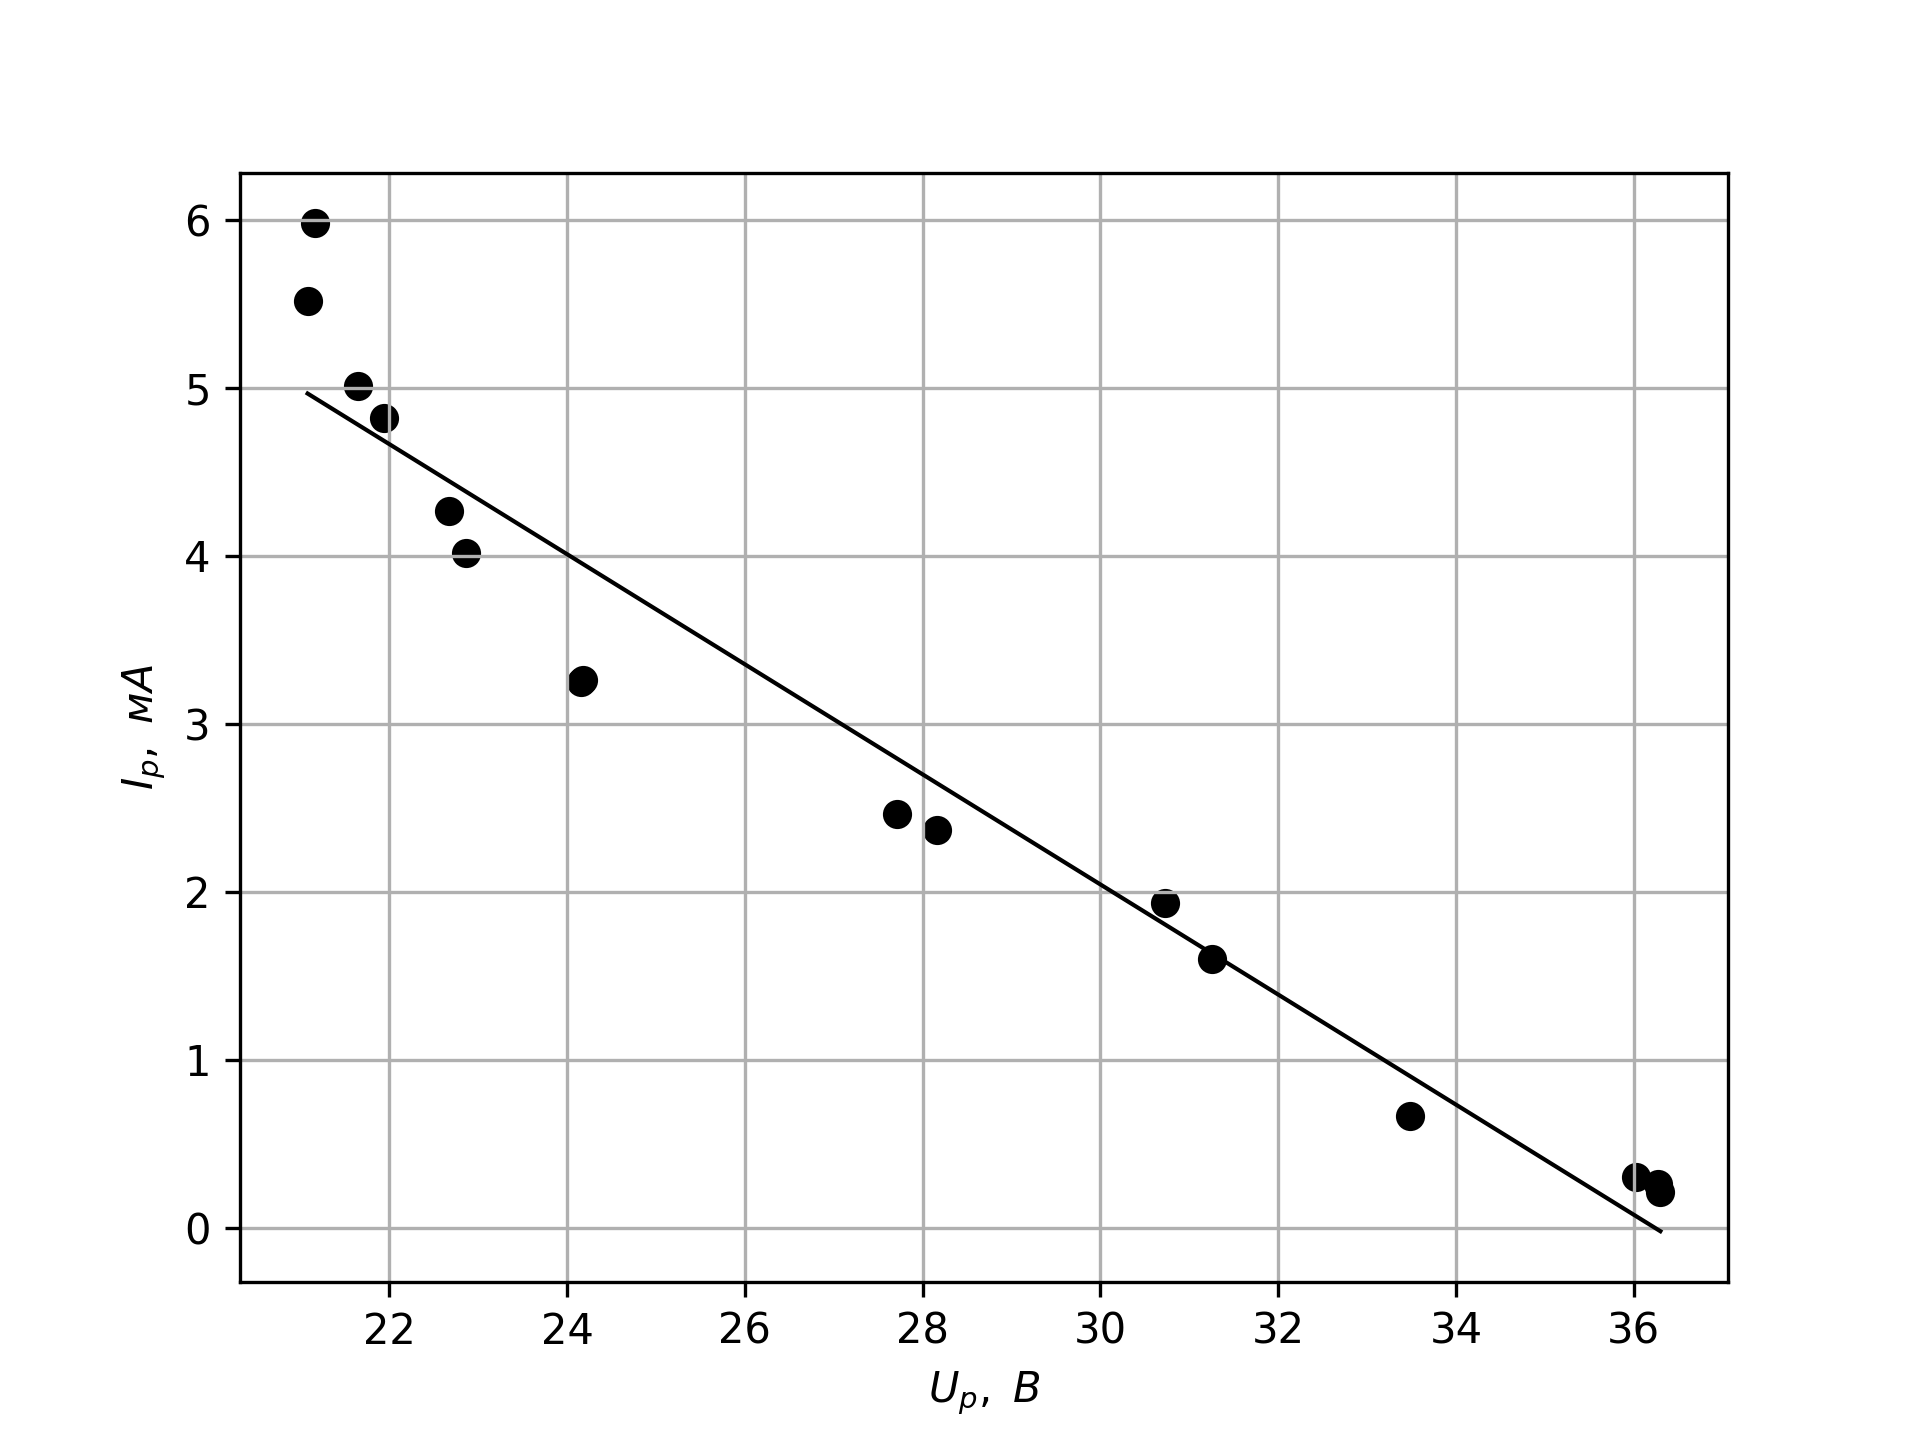
\includegraphics[scale=0.6]{images/351_1.png}
\caption{Вольт-амперная характеристика разряда $I_р(U_р)$}
\end{figure}

\begin{figure}[h]
\centering
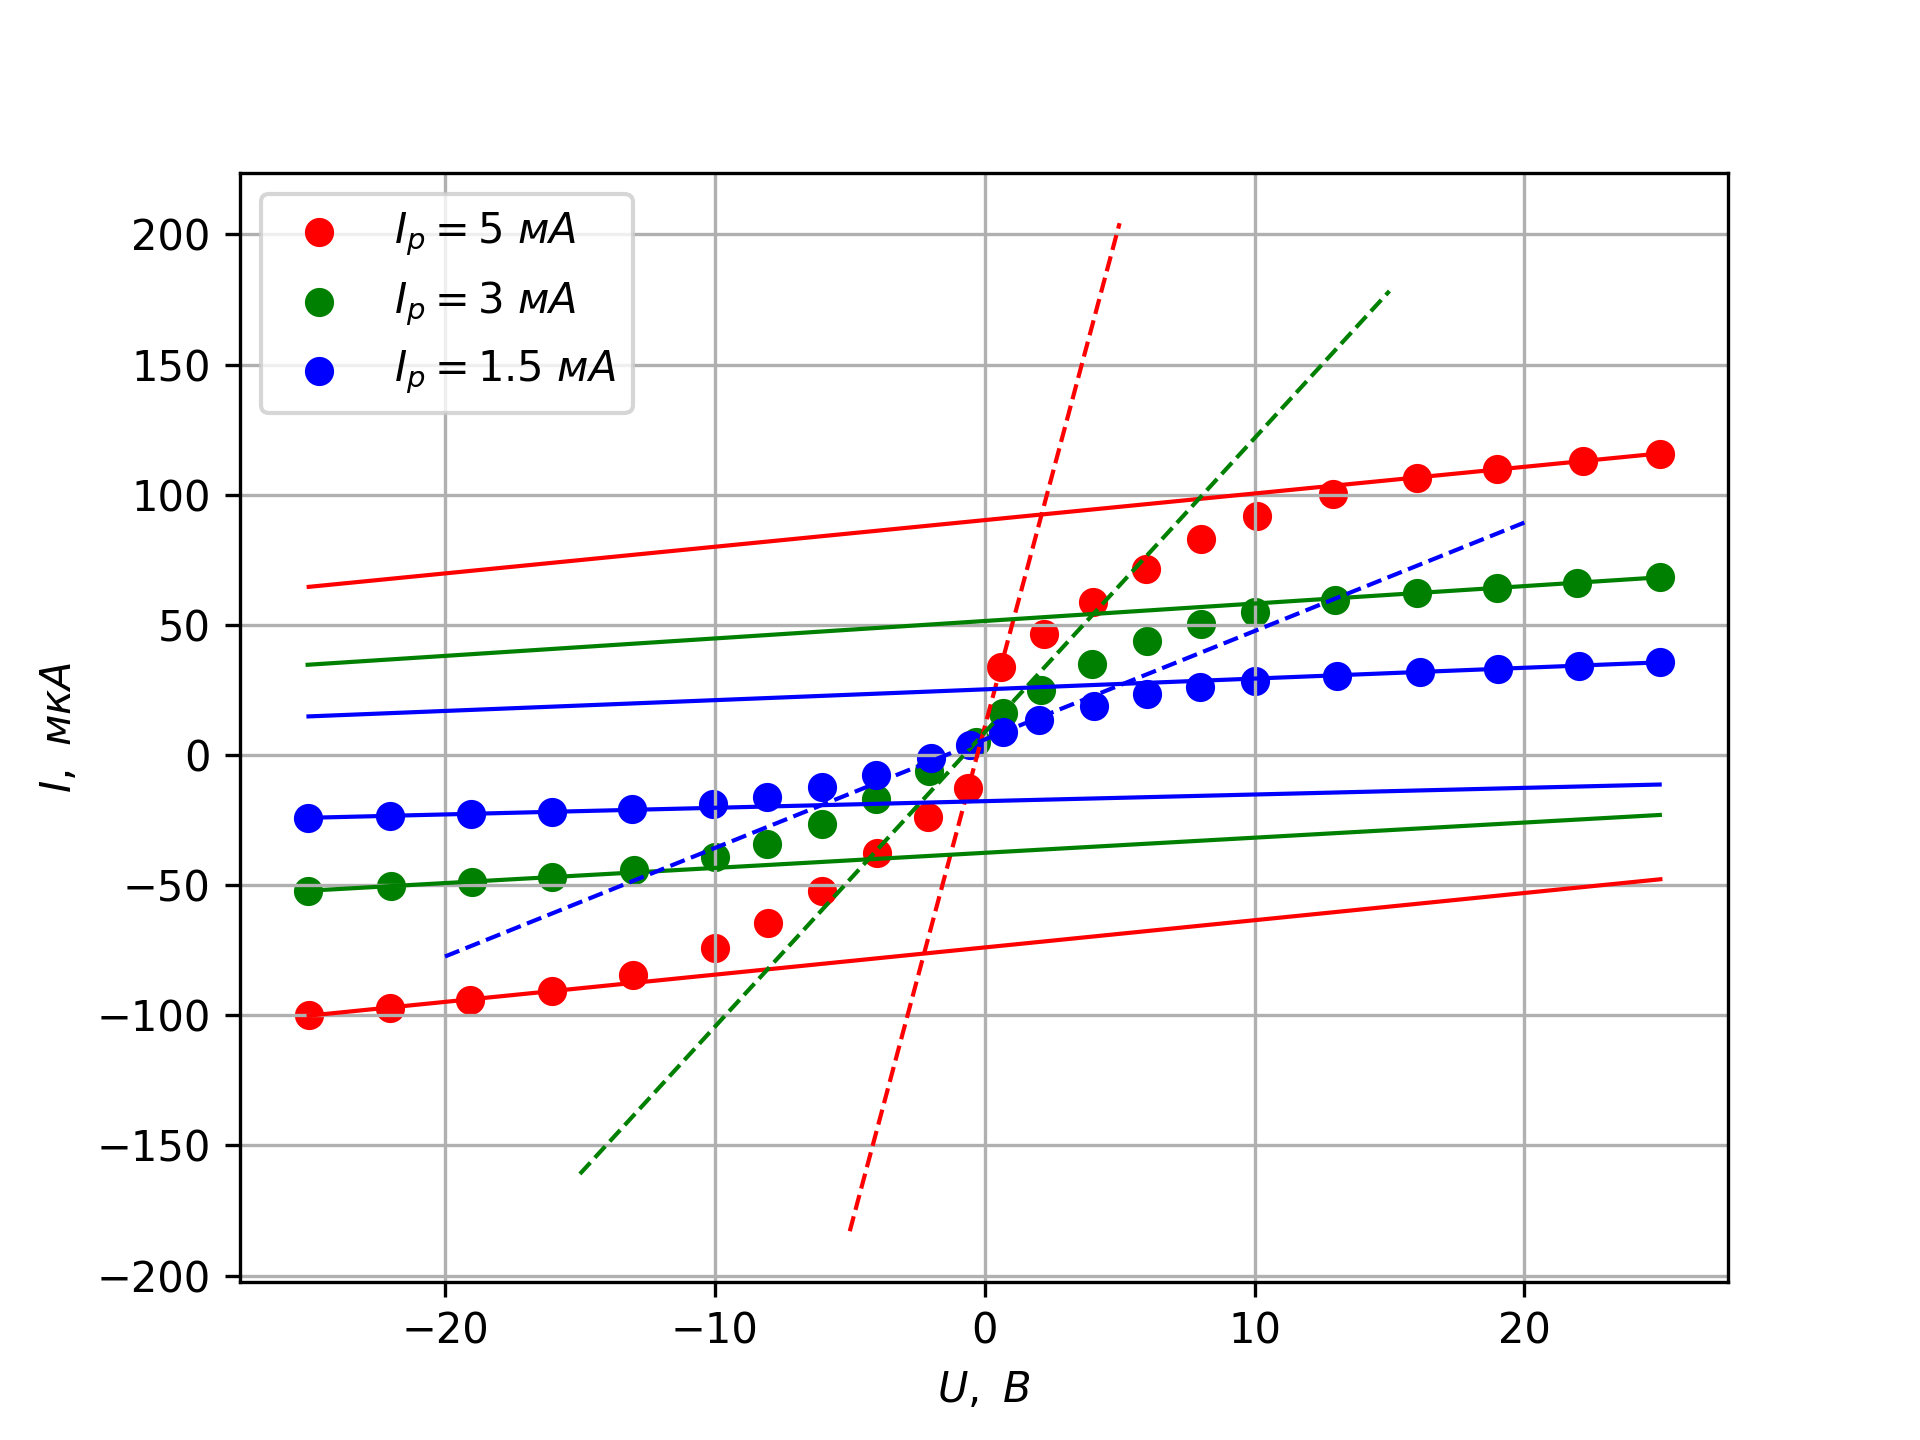
\includegraphics[scale=0.6]{images/351_2.png}
\caption{Вольт-амперная характеристика зонда для разных токов разряда $I(U)$}
\end{figure}

\begin{figure}[h]
\centering
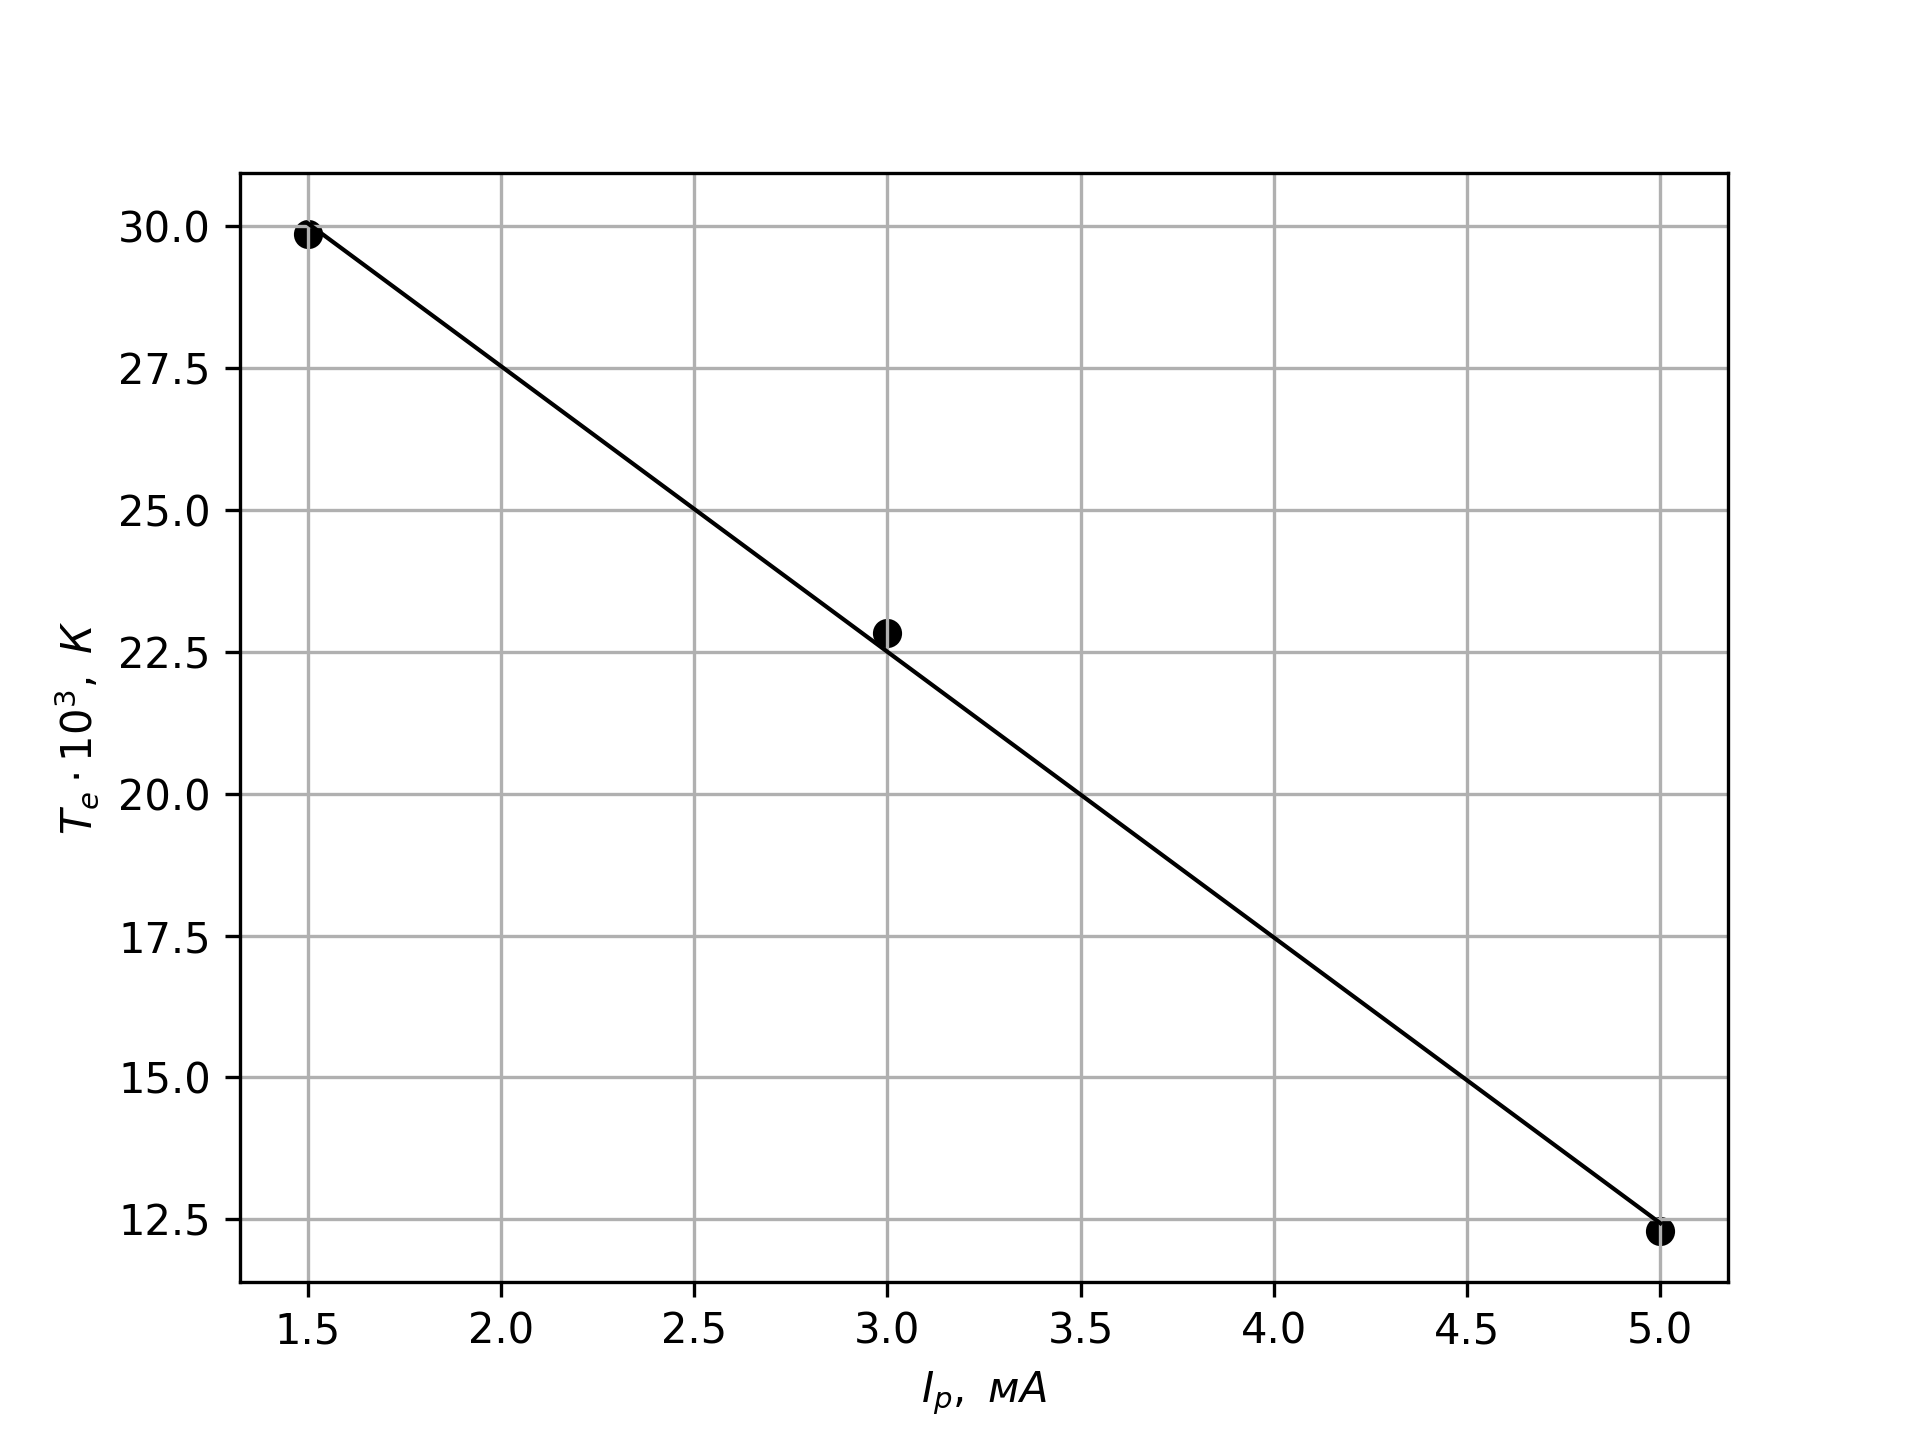
\includegraphics[scale=0.6]{images/351_3.png}
\caption{Зависимость $T_e(I_р)$}
\end{figure}

\begin{figure}[h]
\centering
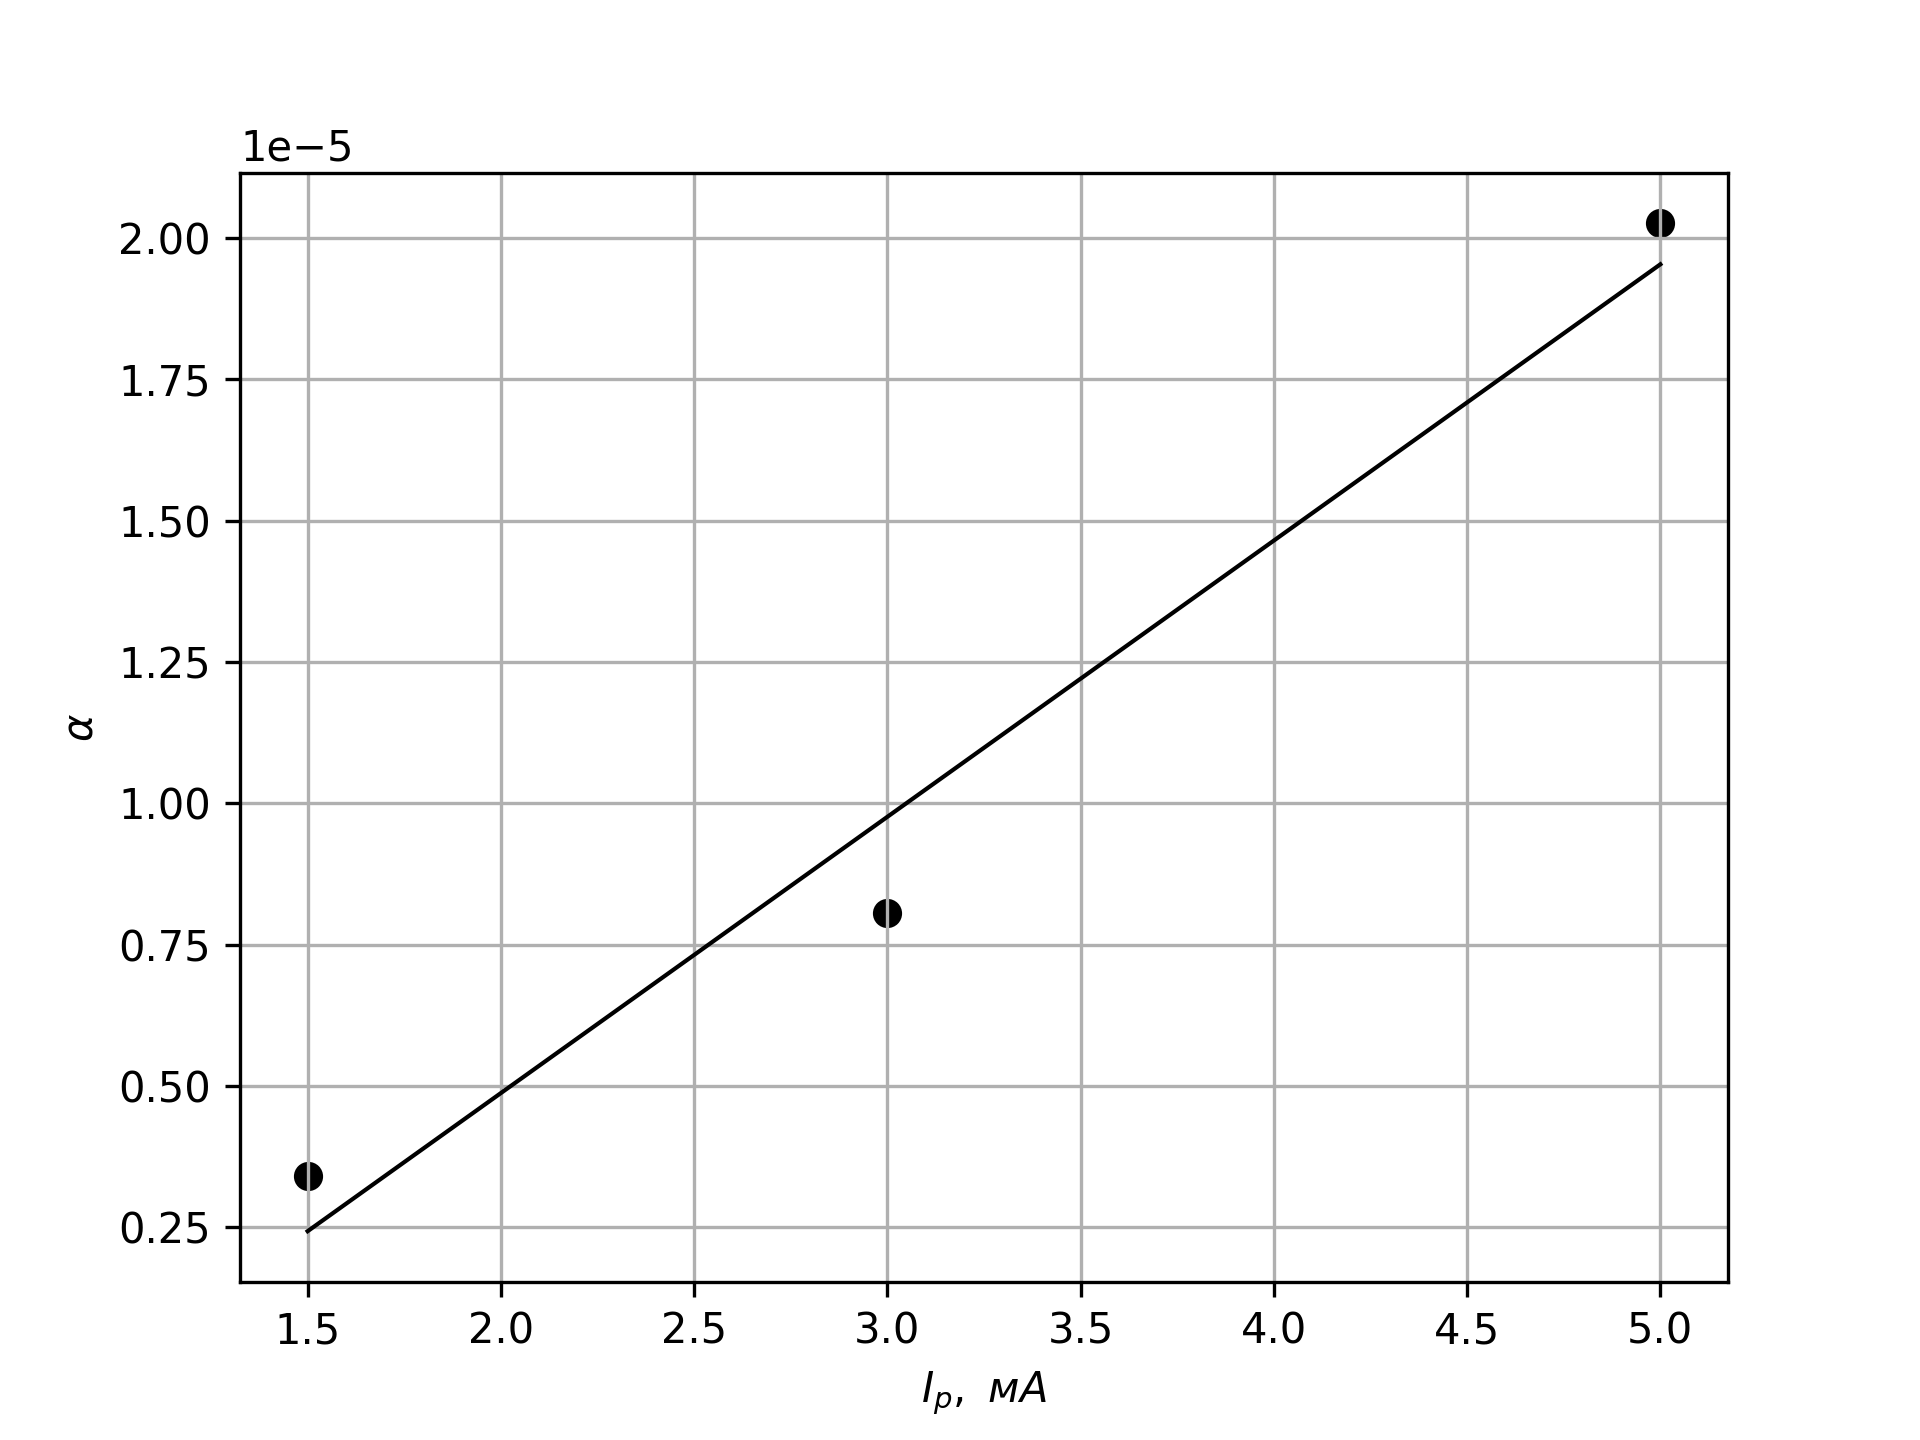
\includegraphics[scale=0.6]{images/351_4.png}
\caption{Зависимость $\alpha(I_р)$}
\end{figure}


\end{document}